\documentclass[final,3p,times,twocolumn]{elsarticle}

\makeatletter
\def\ps@pprintTitle{%
   \let\@oddhead\@empty
   \let\@evenhead\@empty
   \let\@oddfoot\@empty
   \let\@evenfoot\@oddfoot
}
\makeatother

\usepackage{graphicx}
\usepackage{amssymb}

\begin{document}

\begin{frontmatter}

\title{Accounting for Changes in Existing Connections in the Preferential Deletion Model for Web-Like Networks}
\author{Carlos Santiago Bañón}
\address{College of Engineering and Computer Science - University of Central Florida - Orlando, FL}

\begin{abstract}
This paper presents a new \textit{Preferential Deletion Model with Changes in Existing Connections (PDCModel)} that can be used to better study the behavior of real-life social networks. It uses the \textit{Preferential Deletion Model} defined by Narsingh Deo and Aurel Cami in their 2005 paper \textit{Preferential Deletion in Dynamic Models of Web-Like Networks} and expands upon it. We then analyze a dynamic graph randomly generated by our new \textit{PDCModel}, and explore its number of nodes, number of edges, average degree, and degree distributions. When analyzing this new degree distribution, it is evident that it peeks at a degree of $k = 6$, which differs significantly with the original model. Therefore, we can conclude that the average number of connections in social accounts actually peaks at $k = 6$, and not $k = 1$ as presented by Deo and Cami in their paper.
\end{abstract}

\begin{keyword}
Web-Like Networks \sep Interconnection Networks \sep Dynamic Random Graph Modeling \sep Preferential Node Deletion \sep Scale-Free \sep Power-Law Degree Distribution \sep Social Networks \sep Changes in Existing Edges
\end{keyword}

\end{frontmatter}

\section{Introduction}
\label{S:1}

When studying networks, the term \textit{web-like} is often used to refer to tangible, real networks that are not random in nature. These networks can have many applications in various fields, such as telephone networks, neural networks, and social networks. This paper focuses on the latter. The study of how social networks behave is essential for understanding today's world, as there is a parallel between real-life connections from person to person and the same connections in the context of social networks such as Facebook, Instagram, Twitter, and others.

To study social networks, many models have been proposed throughout the years. All of these employ the study of graph theory, a very unique, yet essential area of study within the field of computer science. To represent these networks using graphs, we can simply use nodes as accounts in the network and edges as connections, or friendships between these accounts.

This paper provides a new model that can be useful in the study of these networks. In order to arrive to the creation of our new model, another interesting model developed by Narsingh Deo and Aurel Cami in 2005 was first examined. Their model, called the \textit{Preferential Deletion Model}, seeks to also provide a thorough understanding of real-life networks, and is the basis of our new model.$^{[1]}$

In their paper \textit{Preferential Deletion in Dynamic Models of Web-Like Networks}, they include a very important discussion that can help understand how to create such models. They first state that the Erdös-Rényi model does not provide an accurate picture for these networks, which is a model that develops completely randomized dynamic graphs.$^{[1]}$ Therefore, they established their model with preferential deletion, which is defined in Section 3.

However, their model only accounts for the creation and deletion of nodes. It does not study the case where existing connections between nodes are changed throughout the life cycle of the network. For example, modern social networks give users the ability to friend existing accounts. Therefore, the new model proposed in this paper seeks to evaluate the case where new connections are created between existing nodes.

This new model, described as a \textit{Preferential Deletion Model with Changes in Existing Connections}, is defined in Section 4, and the rest of the paper serves to compare both models, particularly their degree distributions.

\section{Notation}
\label{S:2}

The notation used throughout this paper is outlined in Figure 1.

\begin{figure}[h]
\centering
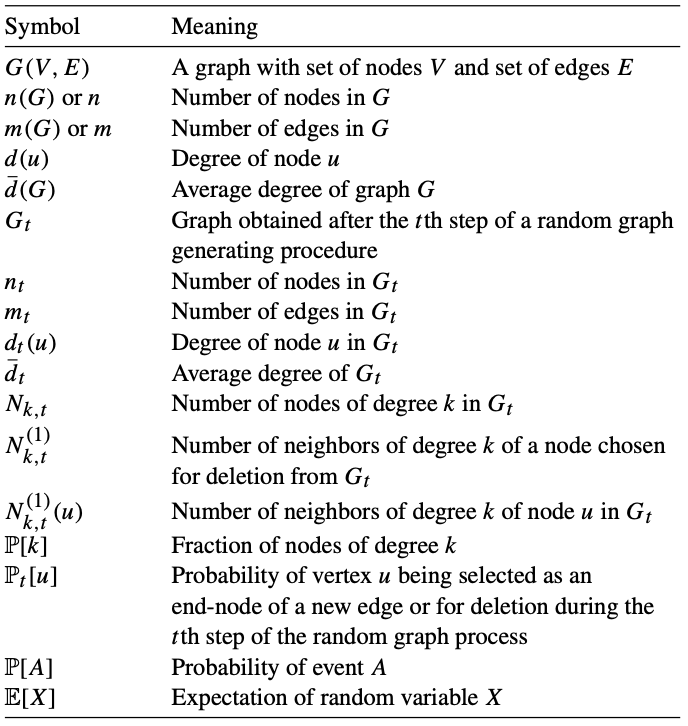
\includegraphics[width=1\linewidth]{notation.png}
\caption{List of symbols.}
\end{figure}

\section{Definition of the Preferential Deletion Model (\textit{PDModel})}
\label{S:3}

Let $G_1$ be a graph that begins with a single node and a self-loop. For each discrete time step $t + 1$, $t > 0$, either one of these processes can occur:

\subsection{Birth Process}

Deo and Cami define the birth process as follows: with probability $p$, a new node is added, together with a new edge incident on it. The other end-node $u$ of the new edge is chosen preferentially from among all the existing nodes based on a \textit{linear preferential attachment rule}.$^{[1]}$

This linear preferential attachment can be defined as:

\begin{equation}
\centering
    \mathbb{P}_{t + 1}[u] = \frac{d_t(u)}{\sum_{w \in V_t} d_t(w)} = \frac{d_t(u)}{2m_t}.
\end{equation}

\subsection{Death Process}

If a new node is not created, then a node will be deleted from the list. This process is defined as follows: with probability $q = 1 - p$, a node $u$ is chosen for deletion along with all the edges incident on it in $G_t$. To make small-degree nodes more likely candidates for deletion than the higher-degree ones, node $u$ is chosen according to the probability distribution defined below.$^{[1]}$

\begin{equation}
\centering
    \mathbb{P}_{t + 1}[u] = \frac{n_t - d_t(u)}{n^2_t - 2m_t}
\end{equation}

Finally, they state that, if during any step $t < 0$, the graph becomes empty, then it starts anew with a single node and a self-loop.

\section{Definition of the Preferential Deletion Model with Changes in Existing Nodes (\textit{PDCModel})}
\label{S:4}

To define this new model, extensive research was made to paint an accurate picture of how social networks behave and evolve.

Therefore, this new model uses the original \textit{Preferential Deletion Model} as a foundation and builds on it. To account for new connections, the following question had to be answered first: \textit{What is the probability that a given two people will meet?} In their paper \textit{The Structure of Growing Social Networks}, Emily M. Jin, Michelle Girvan, and M.E.J. Newman provide an excellent answer to this question, formally providing a thorough mathematical answer.$^{[2]}$

Therefore, the probability per unit time $p_{ij}$ of a given two people $i, j$ meeting is:

\begin{equation}
\centering
    p_{ij} = f(d_i)f(d_j)g(z_{ij}),
\end{equation}

where $d_i$ and $d_j$ are the degrees of $i$ and $j$, respectively, and $z_{ij}$ is their number of mutual connections.

Further, they use the \textit{Fermi} function to define $f(d_i)$. In the world of physics, the \textit{Fermi} function models the probability that an electron energy state will be occupied at a particular temperature $T$.$^{[2]}$ However, they found that it can be very useful in this context. Thus, they formally define $f(d_i)$ as 

\begin{equation}
\centering
    f(d_i) = \frac{1}{e^{\beta(d_i - d*) + 1}},
\end{equation}

where $d*$ is a parameter that makes the equation fall sharply if large, and $\beta$ is a temperature-like arbitrary value that controls such sharpness.

As for $g(z)$, the function serves to show the increase we can expect in the likelihood that two people if they have one or more mutual friends, and is defined as such:

\begin{equation}
\centering
    g(z) = 1 - (1 - p_0)e^{-\alpha z},
\end{equation}

where $p_0$ represents the probability of two people meeting with no mutual acquaintances, and $\alpha$ is a parameter that controls the rate at which the function increases.

This new model creates a new degree distribution that presents a more accurate representation of modern-day \textit{web-like} structures as they relate to social media networks. Further, this paper also analyzes the expected number of nodes, the number of neighbors, the average degree of a graph $G$ created using this new model, and its degree distribution.

\section{Number of Nodes}
\label{S:5}

Upon using this model, the first important conclusion drawn is that the expected number of nodes in graphs $G_1$ and $G_2$ created using the \textit{PDModel} and the \textit{PDCModel}, respectively, is roughly the same. This suggest that the order of growth for both is:

\begin{equation}
\centering
    \mathbb{E}[n_t] = \Theta[(p - q)t].^{[1]}
\end{equation}

Further, as the original paper discusses, the expected number of nodes in both resulting random graphs seldom vanish. That is, there is a very low probability $\mathbb{P}[n_t = 0]$, that the graph will disappear after some step $t > 0$.$^{[1]}$

To better visualize this, Figure 2 shows the expected number of nodes obtained from the new \textit{PDCModel}, and Figure 3 shows a comparison between both the old \textit{PDModel} and the new \textit{PDCModel}.

\begin{figure}[h]
\centering
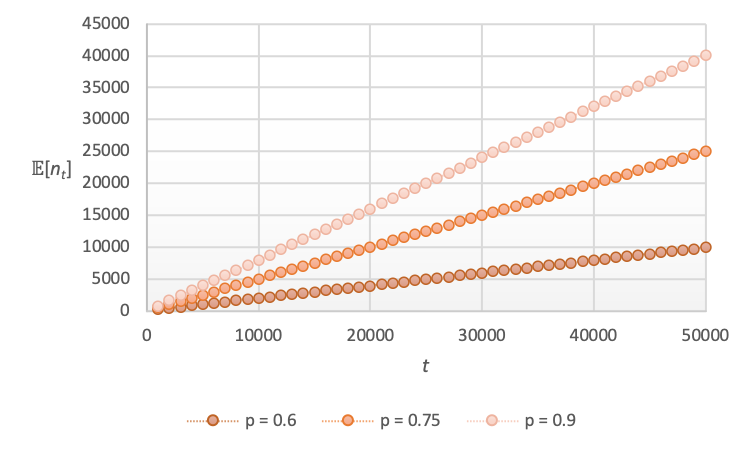
\includegraphics[width=1\linewidth]{nodes.png}
\caption{Expected number of nodes using the new \textit{PDCModel}.}
\end{figure}

\begin{figure}[h]
\centering
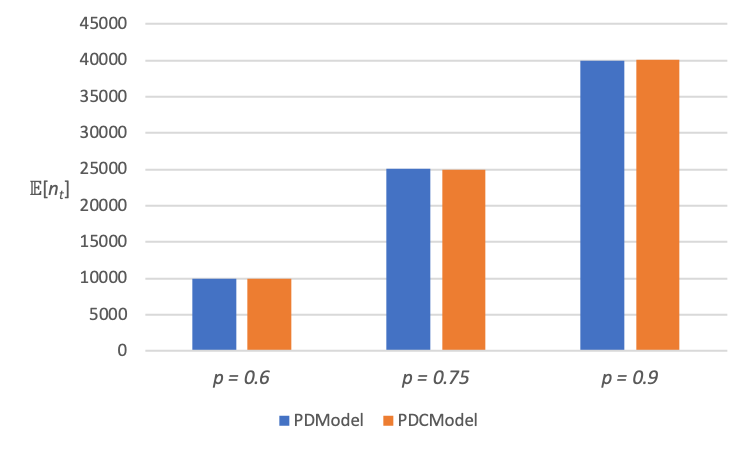
\includegraphics[width=1\linewidth]{nodes-comparison.png}
\caption{Comparison of the expected number of nodes using both the \textit{PDModel} and the new \textit{PDCModel}.}
\end{figure}

\section{Number of Edges}
\label{S:6}

When analyzing the expected number of edges when generating a graph with the new \textit{PDCModel}, this is where the first major change can be observed. Overall, the new model provides graphs with a much higher number of edges. This is due to the nature of the new model, as it continually connects existing nodes throughout the life cycle of the graph. Figure 4 shows how the number of expected edges as $t$ increases.

In addition, Figure 5 shows a comparison between the old and new models. As it is evident, the expected number of nodes is significantly higher in the new \textit{PDCModel}.

\begin{figure}[h]
\centering
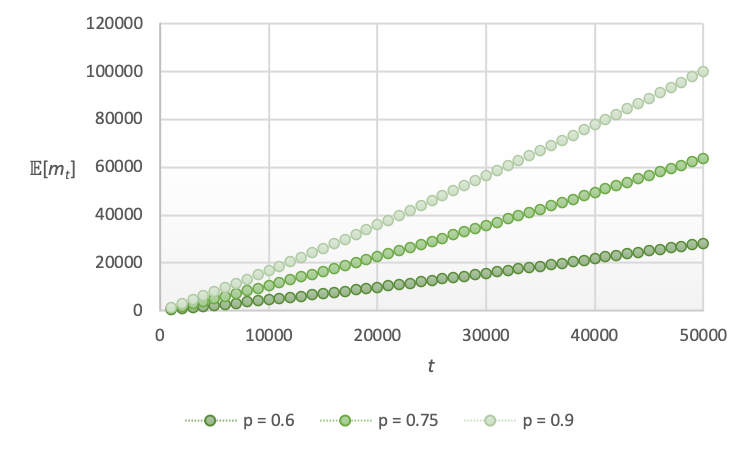
\includegraphics[width=1\linewidth]{edges.png}
\caption{Expected number of edges using the new \textit{PDCModel}.}
\end{figure}

\begin{figure}[h]
\centering
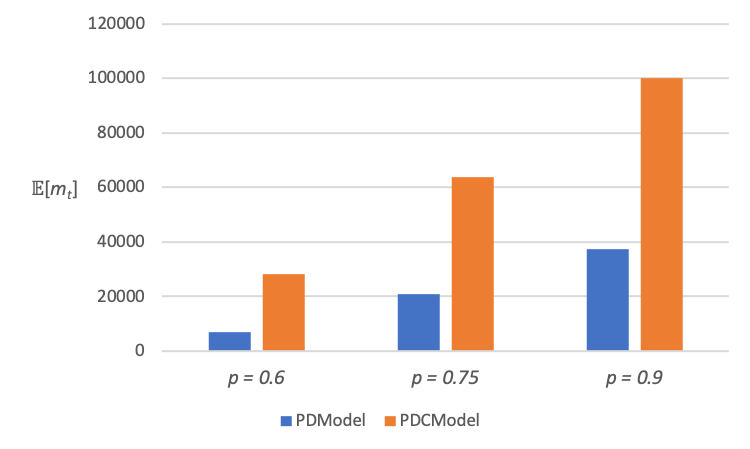
\includegraphics[width=1\linewidth]{edges-comparison.png}
\caption{Comparison of the expected number of edges using both the \textit{PDModel} and the new \textit{PDCModel}.}
\end{figure}

\section{Degree Distribution in the First Neighborhood of the Deleted Node}
\label{S:7}

We then turn to the degree distribution of a random graph $G$ generated with the new model. First, we focus on the degree distribution in the first neighborhood of a deleted node in $G_t$. Deo and Cami formally define this idea as the expected number of neighbors of degree $k$ of a node chosen for deletion from $G_t$.$^{[1]}$ This is where the new model also significantly differs from the old model.

Figure 6 shows the expected number of neighbors of degree $k$ of a node chosen for deletion in a graph generated by the new \textit{PDCModel}. An interesting observation is that the peak in the expected number of neighbors does not occur in degree $k = 1$, as it does in the original \textit{PDModel}. Instead, it peaks at roughly $k = 6$, and subsequently falls sharply. This is again due to the nature of the model itself. It can be concluded that most nodes peak at a degree of at most $k = 6$, and thus it can be difficult to find many nodes with more connections than that.

\begin{figure}[h]
\centering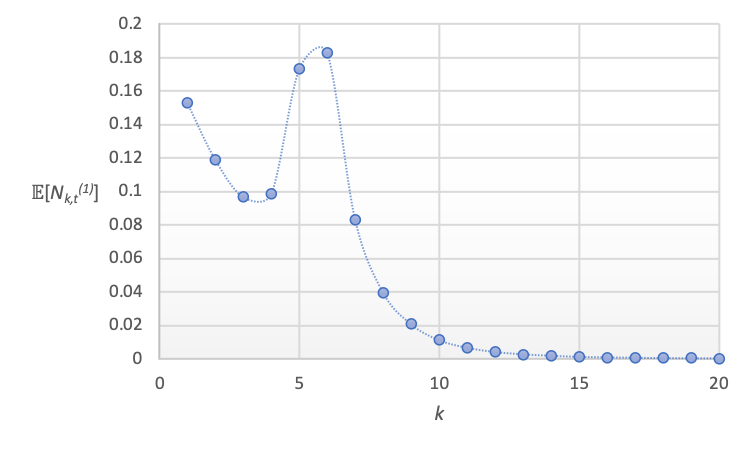
\includegraphics[width=1\linewidth]{degree-distribution.png}
\caption{The expected number of neighbors of degree $k$ of a node chosen for deletion using the new \textit{PDCModel}.}
\end{figure}

Further, Figure 7 shows a comparison of the expected number of neighbors with graphs generated by both the \textit{PDModel} and the \textit{PDCModel}. Here, it is very evident that the peaks are different, due to the definition of both models.

\begin{figure}[h]
\centering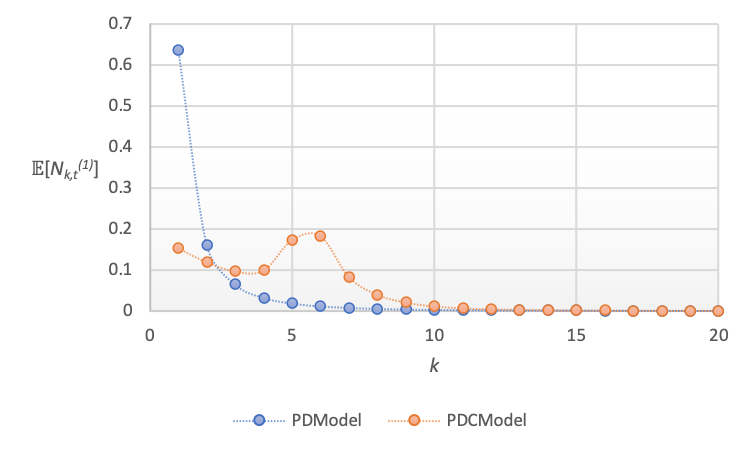
\includegraphics[width=1\linewidth]{degree-distribution-comparison.png}
\caption{Comparison of the expected number of neighbors of degree $k$ of a node chosen for deletion using both the \textit{PDModel} and the new \textit{PDCModel}.}
\end{figure}

\section{Degree Distribution}
\label{S:8}

In terms of the degree distribution of the new \textit{PDCModel}, the results are very similar to those in Section 7. The cumulative degree distribution obtained by the new model can be seen in Figure 8, and it is evident that the same peak phenomenon occurs. The number of nodes of degree $k$ seems to peak at around $k = 6$, again due to the definition of the model itself. Figure 9 then shows a comparison between the old and new models.

\begin{figure}[h]
\centering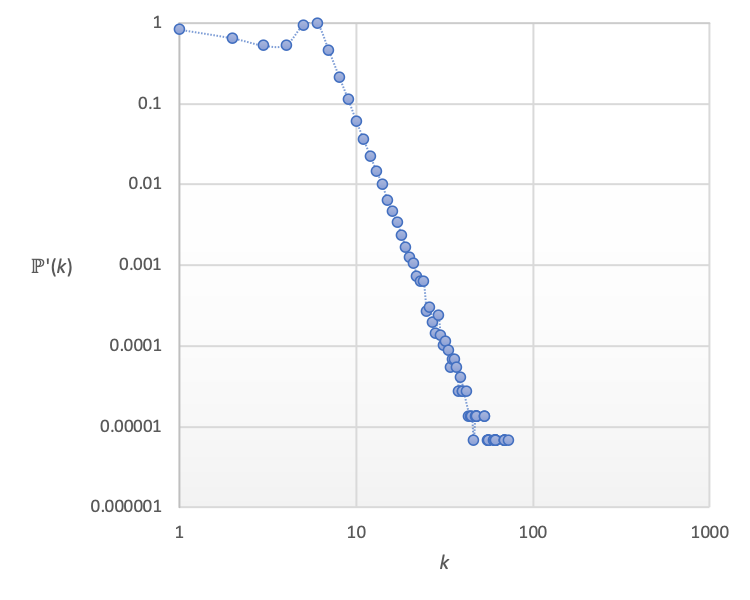
\includegraphics[width=1\linewidth]{cumulative-distribution.png}
\caption{Cumulative degree distribution of the graph generated by the new \textit{PDCModel}.}
\end{figure}

\begin{figure}[h]
\centering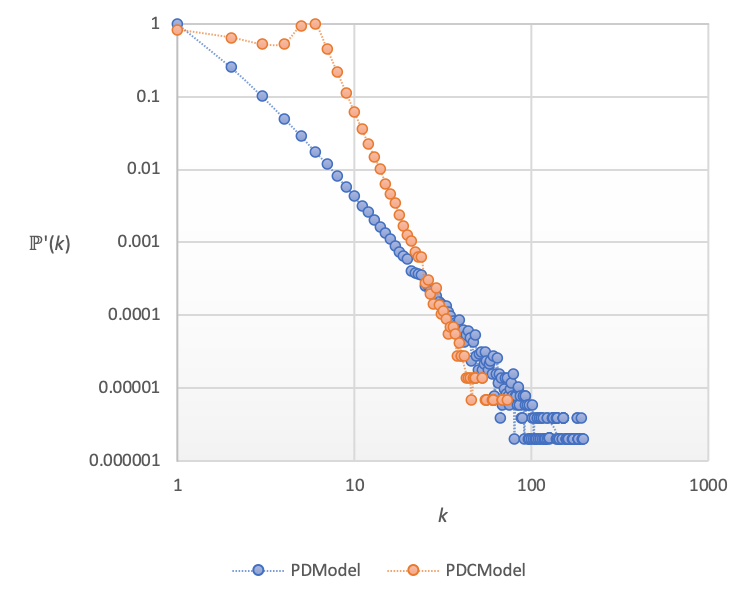
\includegraphics[width=1\linewidth]{cumulative-distribution-comparison.png}
\caption{Comparison of the cumulative degree distributions in graphs generated by both the \textit{PDModel} and the \textit{PDCModel}.}
\end{figure}

\section{Average Degree and Number of New Connections}
\label{S:9}

Another interesting difference we can see between both models is the average degree of a given node in the graphs generated by both models. The average degree is much higher in the graph generated by the \textit{PDCModel}. Figure 10 shows this relationship.

\begin{figure}[h]
\centering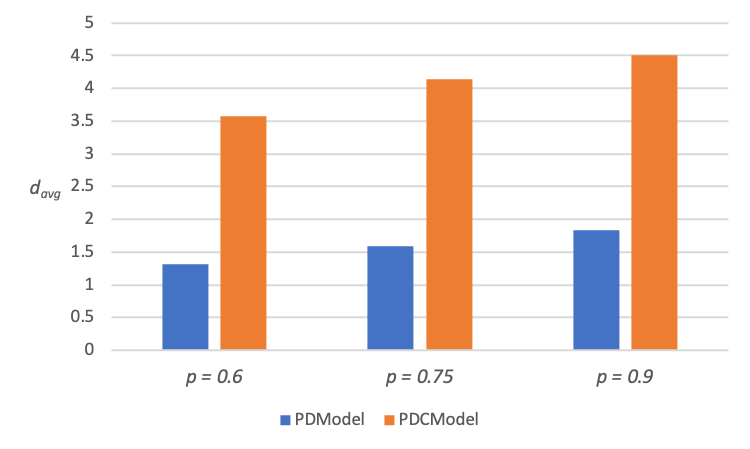
\includegraphics[width=1\linewidth]{average-degree-comparison.png}
\caption{Comparison of the average degree in graphs generated by both the \textit{PDModel} and the new \textit{PDCModel}.}
\end{figure}

Finally, we can take a look at the number of new connections made by the model. As the value of $p$ increases, we can see a sharp increase in the number of additional connections made between existing edges using the \textit{PDCModel}. Figure 11 helps visualize this.

\begin{figure}[h]
\centering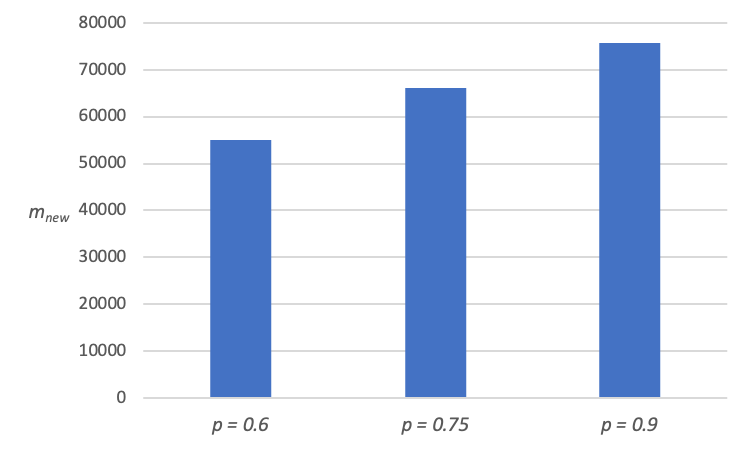
\includegraphics[width=1\linewidth]{edges-growth.png}
\caption{The number of extra edges created by the new \textit{PDCModel}.}

\end{figure}

\section{Conclusion}
\label{S:10}

With this paper, we can conclude that indeed the new \textit{PDCModel} produces different results when compared to the original \textit{Preferential Deletion Model} developed by Deo and Cami. This new model presents a degree distribution that paints a much more accurate picture of the behavior of accounts in social networks. Dynamic graphs generated with the new model produce degree distributions that peak at around $k = 6$, which differs significantly with the original model. Therefore, we can conclude that the average number of connections in social accounts actually peaks at $k = 6$, and not $k = 1$ as presented by Deo and Cami in their paper. This then establishes this model as a sound way of dynamically generating random graphs for further study of \textit{web-like} networks.

\section{References}
\label{S:11}

$[1]$ N. Deo, A. Cami, Preferential deletion in dynamic models of web-like networks, in: Information Processing Letters, Volume 102, Issue 4, 2007, Pages 156-162.

$[2]$ E.M. Jin, M. Girvan, M.E.J. Newman, The structure of growing social networks, in: American Physical Society, Volume 64, Issue 4, 2001, Pages 1-9.

\end{document}
